	\chapter{绪论}
\section{钛工业的发展历程与国内外现状}
\subsection{引言}

钛(Titanium),原子序数为22,最早于1791年由格雷戈尔在英国康沃尔郡发现,是一种银白色的金属,具有密度小、比强度高、耐高温、化学性质性质稳定等明显优于传统金属的特性而备受重视。钛及钛合金常用来制造飞机、火箭等航天机械,一直以来都是航空航天工业的“脊柱”之一,被誉为“太空机械”\cite{XJYS200102014}。与纯钛一同发展起来的钛合金也毫不逊色,钛合金是在纯钛的基础上添加了各种各样的合金元素而形成的合金,凭借其更高的强度、耐蚀性、抗高温性能,得到了广泛的应用,尤其是在机械制造、航空航天、化工、军工等领域,钛合金的占比更大。钛工业的发展水平在一定程度上是衡量一个国家航空航天、汽车工业等发展水平的重要标志\cite{HSJJ202109005}。

\subsection{钛与钛合金的特点}
钛合金具有密度小,强度高的显著特点,相较于高强度钢而言,不仅强度相差无几,而且还具有更大的比强度。

\begin{table}[htbp]
	\centering
	\label{sec:bqd}
	\caption{不同合金比强度比较表}
	\begin{tabular}{ccccc}
		\hline
		\textbf{合金} & \textbf{镁合金} & \textbf{铝合金} & \textbf{高强钢} & \textbf{钛合金} \\
		\hline
		比强度 & 16 & 21 & 23 & 29 \\
		\hline
	\end{tabular}
\end{table}

钛合金的特点如下\cite{1997titanium}:
\begin{enumerate}
	\item 熔点高,钛的熔点为1668℃,比铁的熔点还高出138℃。加入合金元素后可以获得极佳的热强性。
	\item 弹性模量低,屈服强度高,适合做弹簧材料,高端赛车内部的弹簧大多数都是由钛合金制成,它同时还具有较好的耐磨性。
	\item 表面极易生成致密的氧化层,在氧化性或中性介质中有较强的耐腐蚀能力。
	\item 此外还有无磁性,,形状记忆性等优良特点。
	\item 化学活性高,当钛加热到500℃以上时,氧化膜变得稀松且易脱落,在熔融状态下,极易发生自然。
	\item 此外,某些钛合金还具有储氢、超导、低阻尼性,生物相容性、形状记忆 、 超弹 、高阻尼等特殊功能。
\end{enumerate}

由于钛合金具有以上诸多特点,目前已广泛应用于自动化 、能源 、航空航天 、 医	疗卫生 、 汽车和家电等领域。
\subsection{国外发展}
钛工业的发展充满曲折。从钛元素的发现(1791)到第一次制得较纯的金属钛(1910)经历了120年的历程。又由实验室第一次获得纯钛(1940)到首次进行工业生产,又花费了近30年的时间。
钛在自然界中主要以钛矿石的形式存在,如钛铁矿、金红石(TiO2)等,需要进行精炼(refining)才能获得纯金属。起初,钛的提取是通过高温还原法,但这种方法费时费力,成本高昂。直到了二十世纪四十年代,一种利用氯化钛矿与氯气进行反应来制备四氯化钛,然后通过还原反应(比如Na、Mg等)来得到纯钛的精炼工艺方法终于以其低廉的成本、高效的回收率得到了广泛的商业化应用。

第二次世界大战之后,世界上许多国家都开始意识到钛工业的重要性,钛工业在数年间便迅速发展成为航空、航天、军事等领域的关键材料。1954年,美国成功研发出一种Ti-6Al-4V合金,这种合金在耐热性、强度、塑性、韧性、成形性、可焊性、耐蚀性和生物相容性方面均达到较高水平,使它成为钛工业的主要合金,并占据全部用钛量的50%以上,可以说,许多其他型号钛合金也可以作为Ti-6Al-4V的改良版\cite{COLO200102000}。

\subsection{国内发展}
我国的钛工业发展起源于20世纪50年代,在六七十年代,成为了世界上第四个拥有完整钛工业体系的国家。自21世纪以来我国钛工业进入高速发展阶段,产能与产量已经连续多年占据世界第一的位置,目前海绵钛产量占全球比重已经达到六成,钛加工材产量稳定增长,钛产品消费端需求旺盛\cite{JSTB202209001},无论是在生产还是在加工领域均保持在世界前列,我国已成为名副其实的世界钛工业大国。2014年,浙江余杭高端钛材的研发投产,标志着中国彻底摆脱了对国外的依赖,填补了中国高端钛材的技术空白。\cite{TGYJ200405004}

目前,我国的钛产品消费正处于上升期,如工业、航空航天、海洋船舶和体育休闲等中高端领域的钛材料的需求量平均增长约20%,而医疗行业受疫情影响,需求有所减少,电力和制盐等行业仍有小幅增长,整体盈利水平也有所改善\cite{BJKY202204004}。

此外,近年来计算机技术的发展也为钛工业带来了新的发展机遇。计算机模拟技术用于优化钛合金的生产工艺,显著提高了产品质量。邵一涛等通过采用BP人工神经网络方法建立TC17钛合金组织与性能的关系模型,克服了传统BP人工神经网络训练高精度而预测低精度的过拟合问题\cite{BP};计算机辅助设计和制造技术也为钛制品的设计和生产带来了更多的可能,李淼泉等人对 TC6 合金叶片在等温锻造过程中初生α晶粒尺寸的演变进行了数值模拟\cite{Moni},将有限元法与 Yada 微观组织模型结合起来,并给出了 TC6 合金叶片在等温锻造过程中初生α相的分布和晶粒尺寸的变化。在未来,随着物联网、大数据、人工智能、AIGC等技术的不断发展,钛工业也将迎来更多新的机遇和挑战。
\subsection{应用领域}

进入21 世纪以来,钛工业在多个领域遍地开花。
\begin{itemize}
	\item 	在航空航天领域中,大型客机的研制如火如荼、军机也处于过渡时期,世界航空工业对钛合金的需求也随之迅猛增长。
	\item 在医疗健康领域,由于钛合金生物相容性良好,可以降低人体对植入物的排斥反应和感染风险,它也被广泛用于制造人工关节、牙科种植体和其他医疗设备。
	\item 在汽车制造领域,钛合金的应用主要集中在高档汽车的制造中。钛合金零部件可以减少车辆的自重,从而提高燃油效率和运行性能。同时,钛合金也具有优异的耐腐蚀性能,可以延长汽车零部件的使用寿命。
	\item 在建筑工程领域,钛合金被广泛应用于大型建筑的外墙幕墙、顶棚和立面系统。钛合金具有良好的耐候性和抗腐蚀性能,可以抵御各种恶劣气候条件的侵蚀,并且具有高度的可塑性和装饰性,可以为建筑带来更加优美的外观。

\end{itemize}
\section{钛合金的分类}
由于纯钛的塑性高,但强度很低,限制了其在工业生产中的应用。为了满足实际生产中高强度、耐腐蚀性等要求,可以向纯钛中添加一些合金元素形成钛合金。
\subsection{合金元素}
工业钛合金的主要合金元素为铝、钒、钼三种,此外还有Cr、Mn、Fe、Cu、Sn、Zr、W等元素组成,可以根据合金元素对钛多晶型转变温度的影响可将其分为三大类:$\alpha$稳定元素、$\beta$ 稳定元素、中性元素,形成的四种类型的相图示意图如下:

\begin{figure}[h!]
	\centering
	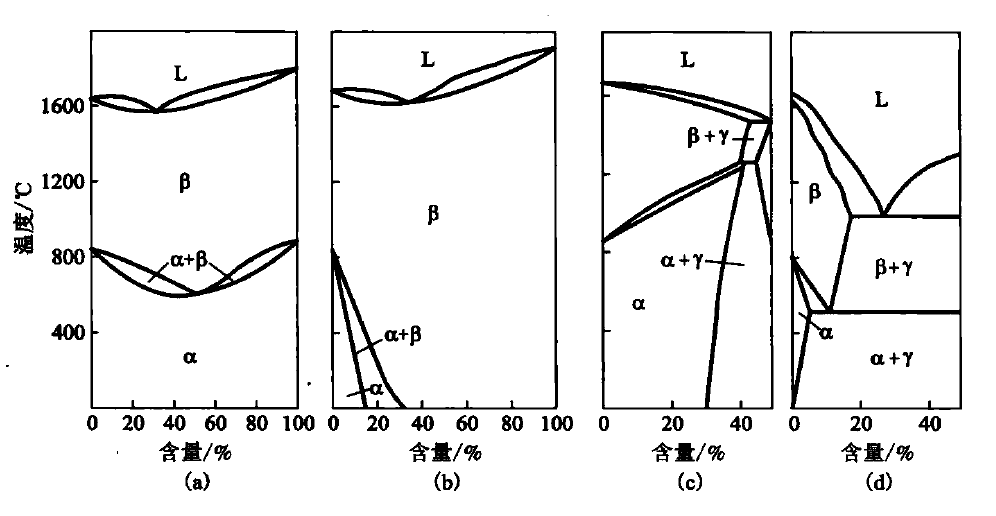
\includegraphics[width=0.9\linewidth]{pic/01}
	\caption{合金元素对钛合金相图的影响示意图}
	\label{fig:01}
\end{figure}
具体来讲,就是根据β相稳定元素系数$K_{\beta}$来划分,$K_{\beta}$是指合金中各β稳定元素与各自的临界浓度的比制之和,即:
$$
K_{\beta}=\frac{ C_{1} }{C_{k1}}+\frac{ C_{2} }{C_{k2}}+\frac{ C_{3} }{C_{k3}}+\cdots+\frac{ C_{n} }{C_{kn}}
$$
根据 $\beta$ 相稳定系数划分合金类型为:
\begin{enumerate}
	\item  $\alpha$ 型合金 $K_\beta$ 为 $0 \sim 0.07$
	\item 近 $\alpha$ 型合金 $K_\beta$ 为 $0.07 \sim 0.25$
	\item $\alpha+\beta$ 型合金 $K_\beta$ 为 $0.25 \sim 1.0$
	\item 近 $\beta$ 型合金 $K_\beta$ 为 $1.0 \sim 2.8$
	\item $\beta$ 型 合金 $K_\beta$ 为 > 2.8
\end{enumerate}
\subsection*{(1)α型}
α型钛合金经退火处理,其组织常以**单相的α固溶体**或者以含微量金属化合物的α固溶体形式存在,主要合金元素为铝、锡、锆等α稳定元素,并少量含有钒、 钼、铌等中性元素,各个元素均可起到固溶强化的作用。

常用的α型钛合金包括TA1、TA2、TA7等。

α型钛合金的β相转变温度较高,因而具有良好的热强性、高温稳定性。焊接性性能好,并在高温环境下具有极好的组织稳定性和抗蠕变性能,在低温环境下也依然保持良好的延展性,因而适合制作各种飞行器形状复杂的外层板材。但它对热处理和组织类型不敏感,故不能采用热处理的方式强化其组织。
\subsection*{(2)β型}
β型钛合金中主要有钒、钼、铌、钽等β相稳定元素,若在合金中加入少量的 铝、锆、锡,可提高β型钛合金的塑性并改善其热稳定性。

常见的β型钛合金有TB1~TB5、TB7、TB10等。

β型钛合金的显微组织 一般比α型、α+β型钛合金的显微组织更粗大。β型钛合金常表现出良好的冷成形、冷加工性能,较好的淬火态塑性以及可焊接性,但是亚稳态β型钛合金热稳定性 较差β型钛合金含有较高的β稳定元素,主要分为稳定β型钛合金和亚稳定β型钛合金。稳定β型钛合金在平衡状态下全部由稳定的β相,热处理后不易产生变化。
\subsection*{(3)α+β型}
α+β型钛合金经退火处理,所得到的室温组织为不同比例的α和β相。该类型的钛合金中除含有定量的铝元素外,还含有少量的其它元素。可采用适当的热处理方法对α+β型钛合金进行组织强化,α+β型钛合金的强度和淬透性随着β相稳定元素含量增加而提高,其锻造和轧制等加工成型性能优于α型、β型钛合金。

最常用的α+β型钛合金包括TC4、TC6、TC12等,其中TC4钛合金(等轴马氏体型两相合金)作为做早被应用的钛合金,该合金以其优越的性能占据了钛工业的大量市场,现在占到 Ti 合金总产量的 50$ \%  $, 占到全部Ti 合金加工件的95$ \% $ 。
\section{钛合金的显微组织}
众所周知,材料的最终性能是由显微组织的形态决定的, 不同的组织对应于不同的力学性能, 而微观组织形态主要取决于合金的化学成分、变形工艺和热处理方式等。

前面提到过:钛合金的基本组织是由密排六方的低温 $\alpha$ 相和体心立方的高温 $\beta$ 相构成。 而且除了少数稳定 $\beta$ 型钛合金之外, 体心立方的高温 $\beta$ 相一般都无法保留到室温, 冷却过程中会发生 $\beta$ 相向 $\alpha$ 相的多晶转变, 以片状形态从原始 $\beta$ 晶界析出。片状组织由片状 $\alpha$ 与片状 $\alpha$ 之间的残余 $\beta$ 相构成, 由于其与母相之间存在着一定的结晶 学位向关系, 称为 $\beta$ 转变组织。片状组织在 $\alpha+\beta$ 两相区承受足够大的塑性变形 后再结晶球化得到等轴组织。因此, 按照晶内 $\alpha$ 相的形状变化, $\alpha+\beta$ 型钓合金 的显微组织大致分为 4 类:

\begin{itemize}
	\item 	等轴组织:在 $\beta$ 转变温度以下 $30 \sim 100{ }^{\circ} \mathrm{C}$ 加热, 经过充分的塑性变形和再结晶退火形成。具有较好的塑性,延伸率和较高的断面收縮率,且抗缺口敏感性和热稳定性最好。综合性能好,使用广泛。
	\item 	网篮组织:在 $\beta$ 区加热或开始变形, 在 $\alpha+\beta$ 两相区的变形量不太大时形成。具有高的持久强度和蠕变强度,在热强性方面具有明显的优势,具有高的断裂韧性、低的疲劳裂纹扩展速率。缺点是塑性和热稳定性较低。
	\item 	双态组织:在 $\alpha+\beta$ 两相区的上部加热或者进行变形可以获得。双态组织兼顾了等轴组织和片状组织的优点, 等轴 $\alpha$ 含量在 $20 \%$ 左右的双态组织具有强度 - 塑性 - 韧性 - 热强性的最佳综合匹配。与片状组织相比, 双态组织具有更高的屈服强度、塑性、热稳定 性和疲劳强度; 与等轴组织相比, 双态组织具有较高的持久强度、蜻变强度和断 裂韧性, 以及较低的疲劳裂纹扩展速率 $\mathrm{d} a / \mathrm{d} N$ 。
	\item 	魏氏组织:在较高温度的 $\beta$ 区加热或变形量不够,时可以形成。魏氏组织具有最高的蠕变抗力、持久强度和断裂韧性, 但是其致命的弱点是塑性低, 尤其是断面收缩率远低于其他组织类型。类似于钢中的过热组织, 在实际生产过程中没有特殊的需求应尽量避免。
\end{itemize}

\begin{table}[htbp]
	\centering
	\label{sec:detial}
	\caption{不同组织的性能}
	\begin{tabular}{ccccc}
		\hline
		机械性能 & 抗拉强度 $ \sigma$ MPa & 延伸率 $\delta\%$ & 冲击韧性& 断裂韧性 \\  \hline
		片层组织 & 1020 & 9.5 & 355.3 & 102 \\
		网篮组织 & 1010 & 13. 5 & 533 & - \\
		双态组织 & 980 & 13 & 434.3 & - \\
		等轴组织 & 961 & 16.5 & 473.8 & 58.9 \\ \hline
	\end{tabular}
\end{table}
\section{钛合金相变}
钛合金中的相变主要包括:多晶转变、共析转变、有序化、亚稳相等稳转变、非等温转变等。

%	众多研究者已将钛合金的相变类型绘制成了一个表格:
%	\begin{table}[htbp]
	%	\centering
	%	\label{sec:change}
	%	\caption{相变过程}
	%		\begin{tabular}{ccc}
		%			\hline
		%			编号 & 相变 & 过程 \\ \hline
		%			I & 淬火过程中$\beta$相的分解 & (1)钛的马氏体:$ \beta $ 	o $\alpha^{'}$ , $\alpha^{"}$\$ \\ \hline
		%	~ & 淬火过程中$\beta$相的分解 & (2)无热\$$\backslash$omega\$相:\$$\backslash$beta $\backslash$to $\backslash$omega\_\{$\backslash$text\{无热}} +$\backslash$beta\$ \\ \hline
%II & 等温转变中$\beta$相的分解 & (1) \$$\backslash$beta($\backslash$beta+$\backslash$alpha)$\backslash$to a\^\{"},a\^\{"}$\backslash$text\{富},a\^\{"}$\backslash$text\{贫}\$ \\ \hline`
%~ & 等温转变中$\beta$相的分解 & (2) \$$\backslash$beta\^\{'}$\backslash$beta$\backslash$text\{富},$\backslash$beta$\backslash$text\{贫}\$ \\ \hline
%III & 残余$\beta$相分解 & (1)      相离析: \$$\backslash$beta\_\{$\backslash$text\{残}} $\backslash$to $\backslash$beta\^\{'}+$\backslash$beta\$ \\ \hline
%\end{tabular}
%\end{table}

\section{钛合金组织分析方法}
\section{小结}
